\subsection{Ring configurations}

The key property of rings is that they seperate a planar graph $G$ into an exterior $M$, a border ring $R$ and an interior $\core$. The concept of a ring $R$ and its interior $\core$ will be used so often that we give it a well-known name.

\begin{definition}
    A planar graph $\confg = R_n + \core$ consisting of a ring $R_n$ and an interior $\core$ is called a \emph{ring configuration} on $R_n$. $\core$ is called the \emph{core} of $\confg$.
\end{definition}

\begin{figure}[!h]
    \centering
        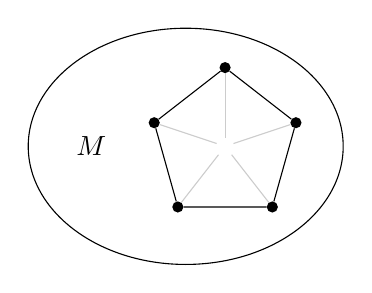
\begin{tikzpicture}
        \draw[fill=white] (-0.5, 0) ellipse (2cm and 1.5cm);
        %\draw[fill=lightgray, draw=black] (0,0) circle (1.25cm);
        %\draw[fill=white] (0,0) circle (0.75cm);
        \node at (-0.7, 0.9) {$\confg$};
        \node at (-1.7, 0) {$M$};

        \node[inner sep=1mm] (c) at (0, 0) {$\core$};
        \node[circle, fill, scale=0.015cm] (l1) at (0, 1) { };
        \node[circle, fill, scale=0.015cm] (l2) at (0.9, 0.30) { };
        \node[circle, fill, scale=0.015cm] (l3) at (0.6, -0.77) {};
        \node[circle, fill, scale=0.015cm] (l4) at (-0.6, -0.77) {};
        \node[circle, fill, scale=0.015cm] (l5) at (-0.9, 0.30) {};

        \draw[opacity=0.2] (c) -- (l1);
        \draw[opacity=0.2] (c) -- (l2);
        \draw[opacity=0.2] (c) -- (l3);
        \draw[opacity=0.2] (c) -- (l4);
        \draw[opacity=0.2] (c) -- (l5);
        \draw (l1) -- (l2) -- (l3) -- (l4) -- (l5) -- (l1);
    \end{tikzpicture}
    \caption{The graph $G=M + \confg$ that contains the configuration $\confg=R_5 + \core$.}
\end{figure}

The idea of $k$-reducibility is that we try to find a \textit{common ring coloring} for $M+R$ and the configuration $\core+R$. If two such colorings can be found, then we can combine both colorings to color $G$. This is exactly a more general approach to what we did for the five color theorem, where the configuration was the vertex $v$ with five neighbors. We can obtain more control over the possible colorings on each side by restricting the ring through the use of a reducer graph $S$. See Figure \ref{fig:reducertut}.

\begin{figure}[!h]
    \centering
    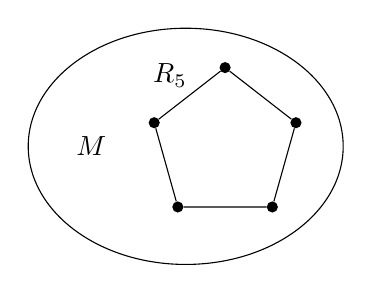
\begin{tikzpicture}
        \draw[fill=white] (-0.5, 0) ellipse (2cm and 1.5cm);
        \node at (-1.7, 0) {$M$};
        \node at (-0.7, 0.9) {$R_5$};

        \node[circle, fill, scale=0.015cm] (l1) at (0, 1) { };
        \node[circle, fill, scale=0.015cm] (l2) at (0.9, 0.30) { };
        \node[circle, fill, scale=0.015cm] (l3) at (0.6, -0.77) {};
        \node[circle, fill, scale=0.015cm] (l4) at (-0.6, -0.77) {};
        \node[circle, fill, scale=0.015cm] (l5) at (-0.9, 0.30) {};

        \draw (l1) -- (l2) -- (l3) -- (l4) -- (l5) -- (l1);
    \end{tikzpicture}
    \hspace{1cm}
    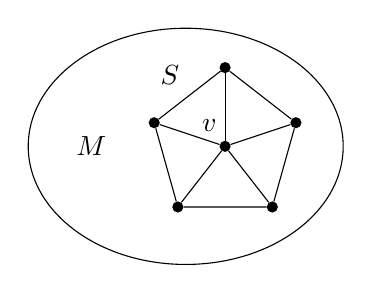
\begin{tikzpicture}
        \draw[fill=white] (-0.5, 0) ellipse (2cm and 1.5cm);
        \node at (-1.7, 0) {$M$};
        \node at (-0.7, 0.9) {$S$};

        \node (c) at (-0.2, 0.27) { $v$ };
        \node[circle, fill, scale=0.015cm] (c) at (0, 0) {};
        \node[circle, fill, scale=0.015cm] (l1) at (0, 1) { };
        \node[circle, fill, scale=0.015cm] (l2) at (0.9, 0.30) { };
        \node[circle, fill, scale=0.015cm] (l3) at (0.6, -0.77) {};
        \node[circle, fill, scale=0.015cm] (l4) at (-0.6, -0.77) {};
        \node[circle, fill, scale=0.015cm] (l5) at (-0.9, 0.30) {};

        \draw (c) -- (l1);
        \draw (c) -- (l2);
        \draw (c) -- (l3);
        \draw (c) -- (l4);
        \draw (c) -- (l5);
        \draw (l1) -- (l2) -- (l3) -- (l4) -- (l5) -- (l1);
    \end{tikzpicture}
    \caption{A graph $M+R_5$ without extra vertices (left). A graph $M+S$ where $S=R_5+v$ (right). The graph $S$ is called a \textit{reducer}.}
    \label{fig:reducertut}
\end{figure}

The colorings of the ring in $M+R_5$ can be any 3-coloring or 4-coloring depending on $M$. However, in the graph $M+S$ it is not possible the color the ring in four colors. Due to the extra vertex introduced by $S$, we are guaranteed to find only 3-colorings on the ring regardless of $M$. An example of such a 3-coloring is $cabab$. This guaranteed 3-coloring is key information in the reducibility proof of $R_5$. 

This reducer can be used in case it is too hard to find a common ring coloring without a restriction. However, the more vertices we use in the reducer, the more vertices we are left with after reducing. By limiting the amount of vertices of the reducer, we can fine-tune how much control we want to have over the colorings. Therefore, let us instead reduce the graph $G=M+R+\core$ to

\begin{equation}
    M+S \;\;\text{and}\;\; \core+S' \quad \text{with} \quad R \subset S,S'.
\end{equation}

For both reducers $S$ and $S'$, we require that $|S| \leq |R| + k$. This parameter has major consequences on the difficulty of our reducibility problem.

\begin{itemize}
    \item If $k=0$, then $S=R$ and we reduce to $M+R$ and $\core+R$. This is the smallest possible reduction and ideal situation.
    \item If $k=1$, then we can set $S=R+v$ like in Figure \ref{fig:reducertut}. Our reduced graph is then one vertex larger. This means that if $M$ or $\confg$ have one vertex, we will not be obtaining any reduction in size. So the result is weaker.
    \item If $k \geq |\confg|$, then there is no point in reducing, since we always obtain the same graph $M+\confg$ or a larger one. Therefore, to obtain a reduction in size, we should also require that $k < |\confg|$. 
\end{itemize}


\begin{definition}
    A configuration $\confg=\core+R$ is \emph{$k$-reducible} if for all planar graphs $G=M+\confg$ and some reducers $S$ and $S'$ on $\leq k < |\confg|$ vertices, there exists a common ring coloring for $M+S$ and $\core+S'$.
\end{definition}
\begin{definition}
    The ring $R_n$ is \emph{$k$-reducible} if all configurations $\confg$ on $R_n$ are at most $k$-reducible.
\end{definition}

A trivial example is the 0-reducibility of the rings $R_2$ and $R_3$. The only possible colorings on these rings are $ab$ and $abc$ respectively. This means that any two colorings of $M+R$ and $\core + R$ are equal up to permutation of colors.
